\documentclass[12pt,a4paper,openany,oneside]{book}
\usepackage{float}
\usepackage{hyperref}
\usepackage[italian]{babel}

\usepackage{xcolor} % Pacchetto per il colore del testo
\usepackage{hyperref} % Pacchetto per i link ipertestuali

% Configurazione del colore dei link ipertestuali
\hypersetup{
    colorlinks=true,
    linkcolor=blue,    % Colore dei link interni
    urlcolor=blue      % Colore dei link URL esterni
}

%\usepackage[latin1]{inputenc} %Windows
\usepackage[utf8x]{inputenc} %Linux
%\usepackage[applemac]{inputenc} %Mac

\usepackage{graphicx}
\usepackage[font=small,labelfont=bf,tableposition=top]{caption}

\usepackage{listings}
  \usepackage{courier}
 \lstset{
         language=C++,
         basicstyle=\footnotesize\ttfamily,
         numbers=left,           
         numberstyle=\tiny,       
         numbersep=5pt,        
         tabsize=5,                 
         extendedchars=true,         
         breaklines=true,
         keywordstyle=\textbf,           
         stringstyle=\color{white}\ttfamily,
         showspaces=false,       
         showtabs=false,           
         xleftmargin=17pt,
         framexleftmargin=17pt,
         framexrightmargin=5pt,
         framexbottommargin=4pt,
         showstringspaces=false          
 }
 
 \addto\captionsitalian{%
 	\renewcommand{\lstlistingname}{Codice}}

\setcounter{tocdepth}{3} % fa apparire le subsubsection nell'indice
\setcounter{secnumdepth}{3} % e le numera


\usepackage{amsmath}


\usepackage{framed}

\begin{document}

%Inserisce qui il frontespizio
\begin{titlepage}
\centering 

\includegraphics[width=2.434cm,height=2.565cm]{Images/university_logo.png}

\bigskip

{\Large \textbf{UNIVERSIT\`A DEGLI STUDI DI CATANIA}}

{\scshape
\large
Dipartimento di Matematica e Informatica
}

{\scshape
\normalsize
Corso di Laurea Triennale in Informatica
}

\bigskip


\hrule


\bigskip


\bigskip


\bigskip


\bigskip

{\itshape
\large
Giulio Pedicone
\par}


\bigskip


\bigskip


\bigskip


\bigskip

{\centering
\Large
Pseudonimizzazione (Attacco)
\par}


\bigskip


\bigskip


\bigskip


\bigskip


\bigskip


\bigskip


\begin{minipage}[b]{8 cm}
\hrule

\bigskip

{\centering\scshape 
Progetto Internet Security
\par}


\bigskip

\hrule
\end{minipage}
\bigskip


\bigskip


\bigskip


\bigskip


\bigskip


\bigskip


\bigskip


\bigskip


\bigskip


\bigskip


\bigskip

{\raggedleft
Prof.re: Giampaolo Bella
\par}


\bigskip


\bigskip


\bigskip


\bigskip

\hrule

\bigskip

{\centering
Anno Accademico 2023 - 2024
\par}
\end{titlepage}
 %<- richiama il file "parts/titlepage.tex" che contiene il frontespizio

%Genera l'indice
\tableofcontents

\chapter{Definizione di Pseudonimizzazione}


La pseudonimizzazione è una tecnica di trattamento dei dati che mira a proteggere la privacy degli individui sostituendo i dati identificativi con pseudonimi. In questo modo, le informazioni originali non possono essere attribuite a una specifica persona senza l'uso di ulteriori informazioni che sono conservate separatamente.

Questa tecnica è utile per ridurre i rischi associati al trattamento dei dati personali, in quanto limita la possibilità di identificare gli individui senza avere accesso alle informazioni aggiuntive necessarie per invertire il processo di pseudonimizzazione.

La pseudonimizzazione è un metodo che permette di sostituire i dati originali (ad esempio, un indirizzo e-mail o un nome) con un alias o pseudonimo. È un processo reversibile che de-identifica i dati, consentendo la re-identificazione in seguito, se necessario. Questa tecnica è altamente raccomandata dal Regolamento Generale sulla Protezione dei Dati (GDPR) come uno dei metodi di protezione dei dati.

\section{Utilizzo della Pseudonimizzazione nella Protezione dei Dati}
La pseudonimizzazione facilita il trattamento dei dati personali, riducendo il rischio di esposizione di dati sensibili a personale e dipendenti non autorizzati.

\subsection{Esempio di utilizzo}
Ad esempio, quando si inviano fogli Excel contenenti dati sensibili via e-mail. Sebbene il mittente e il destinatario delle e-mail siano autorizzati ad accedere a tali informazioni, il supporto IT ha anche accesso a quelle e-mail. Ora immagina che si trattasse di bonus per il top management o informazioni sui salari aziendali. Quando i dati sono pseudonimizzati, c'è meno possibilità di esporre dati personali, poiché i record dei dati diventano non identificabili, rimanendo comunque adatti per l'elaborazione e l'analisi dei dati.

\subsection{Cos'è un Pseudonimo?}
In questo contesto, un pseudonimo è un identificatore associato a un individuo. Proprio come gli scrittori usano pseudonimi per nascondere la loro identità e proteggere la loro privacy, gli pseudonimi vengono utilizzati per lo stesso scopo nella protezione dei dati. Un pseudonimo può essere un numero, una lettera, un carattere speciale o una qualsiasi combinazione di questi legati a un dato personale specifico o a un individuo, rendendo quindi i dati più sicuri da usare in un contesto aziendale. %<- richiama il file "parts/capitolo1.tex" che contiene il primo capitolo
%Si consiglia di creare un nuovo file per ogni capitolo
\chapter{Il GDPR e la Pseudonimizzazione}


\section{Pseudonimizzazione nel GDPR}

L'\textbf{European Union Agency for Cybersecurity} (ENISA) lavora dal 2004 per rendere l'Europa sicura dal punto di vista cibernetico. ENISA collabora con l'Unione Europea, i suoi Stati membri, il settore privato e i cittadini europei per sviluppare consigli e raccomandazioni sulle buone pratiche in materia di sicurezza delle informazioni. Assiste gli Stati membri dell'UE nell'implementazione della legislazione europea pertinente e lavora per migliorare la resilienza delle infrastrutture e delle reti di informazione critiche in Europa. ENISA cerca di potenziare l'esperienza esistente negli Stati membri dell'UE supportando lo sviluppo di comunità transfrontaliere impegnate a migliorare la sicurezza delle reti e delle informazioni in tutta l'UE. Dal 2019, l'ENISA ha elaborato schemi di certificazione della cybersecurity.Lo scorso 3 dicembre, l'European Union Agency for Cybersecurity (ENISA, precedentemente denominata European Union Agency for Network and Information Security) ha pubblicato un importante documento sulla pseudonimizzazione dal titolo \textit{"\textbf{Pseudonymisation techniques and best practices}"} in cui vengono proposti alcuni possibili scenari di attacco a cui sono esposti i nostri dati e le migliori tecniche di difesa oggi in circolazione.

\newpage

\section{Definizione di Pseudonimizzazione nel GDPR}
Nell'Articolo 4(5) del GDPR, i\textbf{l processo di pseudonimizzazione} è definito come:
\begin{quote}
“Il trattamento dei dati personali in modo tale che i dati personali non possano più essere attribuiti a un interessato specifico senza l'utilizzo di informazioni aggiuntive, a condizione che tali informazioni aggiuntive siano conservate separatamente e siano soggette a misure tecniche e organizzative atte a garantire che i dati personali non siano attribuiti a una persona fisica identificata o identificabile.”
\end{quote}

\subsection{Benefici della Pseudonimizzazione secondo il GDPR}
Se sei un Responsabile della Protezione dei Dati (DPO), puoi vedere l'attrattiva e i benefici della pseudonimizzazione. Permette di\textbf{ identificare i dati }se necessario, ma li rende \textbf{inaccessibili agli utenti non autorizzati} e consente ai responsabili e agli incaricati del trattamento dei dati di ridurre il rischio di una potenziale violazione dei dati e proteggere i dati personali.

Il GDPR richiede di adottare tutte le misure tecniche e organizzative appropriate per proteggere i dati personali, e la pseudonimizzazione può essere un metodo appropriato se si desidera mantenere l'utilità dei dati.

\subsection{I Dati Pseudonimizzati sono ancora Dati Personali secondo il GDPR?}
Un pseudonimo è ancora \textbf{considerato un dato personale} secondo il GDPR poiché il \textbf{processo è reversibile} e, con una chiave appropriata, è \textbf{possibile identificare l'individuo}. Il Considerando 26 spiega:
\begin{quote}
“…i dati personali che hanno subito pseudonimizzazione, che potrebbero essere attribuiti a una persona fisica utilizzando informazioni aggiuntive, dovrebbero essere considerati informazioni su una persona fisica identificabile.”
\end{quote}

Inoltre, durante una violazione dei dati, una chiave di crittografia potrebbe essere esposta, mettendo a rischio anche i dati pseudonimizzati.

\section{I Dati Anonimizzati sono ancora considerati Dati Personali?}
Il GDPR si preoccupa solo del trattamento dei dati personali relativi a una persona fisica che consente l'identificazione di un individuo direttamente o indirettamente.

Se i \textbf{dati} sono\textbf{ anonimizzati} in modo che gli individui non possano più essere identificati, il \textbf{GDPR} semplicemente \textbf{non li considera più dati personali}. Tuttavia, l'anonimizzazione dei dati può spesso distruggere il valore che i dati hanno per la tua organizzazione. 
\chapter{Anonimizzazione VS Pseudonimizzazione}

\textbf{Anonimizzazione} e \textbf{pseudonimizzazione} sono tecniche utilizzate per proteggere l'identità degli individui nei dati, ma non sono sinonimi. In questo documento, esploreremo come funzionano entrambe le tecniche e come vengono trattate dal GDPR e dalle raccomandazioni dell'ENISA.

\section{Pseudonimizzazione}
Con la pseudonimizzazione, se sei autorizzato ad accedere a tali informazioni, avrai la chiave che permetterà di \textbf{de-identificare i dati}. La pseudonimizzazione è una tecnica che altera \textbf{reversibilmente} i dati in modo che possano essere riconosciuti in un secondo momento, se necessario.

\section{Anonimizzazione}
L'anonimizzazione è una tecnica che\textbf{ altera irreversibilmente i dati} in modo che un individuo non possa più essere identificato direttamente o indirettamente. 

\newpage

\section{Perché Optare per la Pseudonimizzazione?}
Nelle operazioni quotidiane di qualsiasi azienda, molti dati sensibili passano attraverso i dipartimenti HR, marketing o IT, e la pseudonimizzazione può aiutare a \textbf{ridurre il rischio} e \textbf{prevenire eventuali violazioni dei dati}.

\subsection{Recital 28 del GDPR}
\begin{quote}
“L'applicazione della pseudonimizzazione ai dati personali può ridurre i rischi per gli interessati e aiutare i responsabili e gli incaricati del trattamento a soddisfare i loro obblighi di protezione dei dati.”
\end{quote}

La pseudonimizzazione non solo protegge i dati, ma supporta anche la conformità generale al GDPR di qualsiasi organizzazione.

\section{Raccomandazioni sull'Uso della Pseudonimizzazione e Anonimizzazione}
\subsection{Anonimizzazione}
Si raccomanda vivamente di anonimizzare i dati personali negli ambienti non di produzione, utilizzati per lo sviluppo, il testing e la formazione. 

\subsection{Pseudonimizzazione sui Sistemi di Produzione}
Quando si progetta la protezione dei dati per i sistemi di produzione live, si consiglia di utilizzare la pseudonimizzazione. 

\subsection{Automatizzazione}
Sia la pseudonimizzazione che l'anonimizzazione dovrebbero essere automatizzate, così come le convalide dei dati, per ridurre al minimo gli errori umani.

\subsection{Scelta della Tecnica Appropriata}
Le tecniche utilizzate devono essere applicabili a uno specifico caso d'uso o sistema.


\section{Raccomandazioni dell'ENISA per la Pseudonimizzazione}
L'European Union Agency for Cybersecurity (ENISA) ha pubblicato un rapporto su “Pseudonymisation Techniques and Best Practices”, in risposta alle sfide dell'implementazione della pseudonimizzazione nella pratica.

\subsection{Criteri per la Scelta delle Tecniche di Pseudonimizzazione}
La guida discute i criteri per la scelta delle tecniche di pseudonimizzazione appropriate, come la protezione dei dati, la scalabilità e il recupero. 

\subsection{Conclusioni del Rapporto}
Il rapporto ha concluso che non esiste una soluzione unica che funzioni per tutte le industrie o tutti gli scenari.

\begin{quote}
“…non esiste una soluzione unica e facile alla pseudonimizzazione che funzioni per tutti gli approcci in tutti i possibili scenari. Al contrario, richiede un alto livello di competenza per applicare un processo di pseudonimizzazione robusto, possibilmente riducendo la minaccia di discriminazione o attacchi di re-identificazione, mantenendo il grado di utilità necessario per il trattamento dei dati pseudonimizzati.”
\end{quote}

\begin{figure}[H]
    \centering
    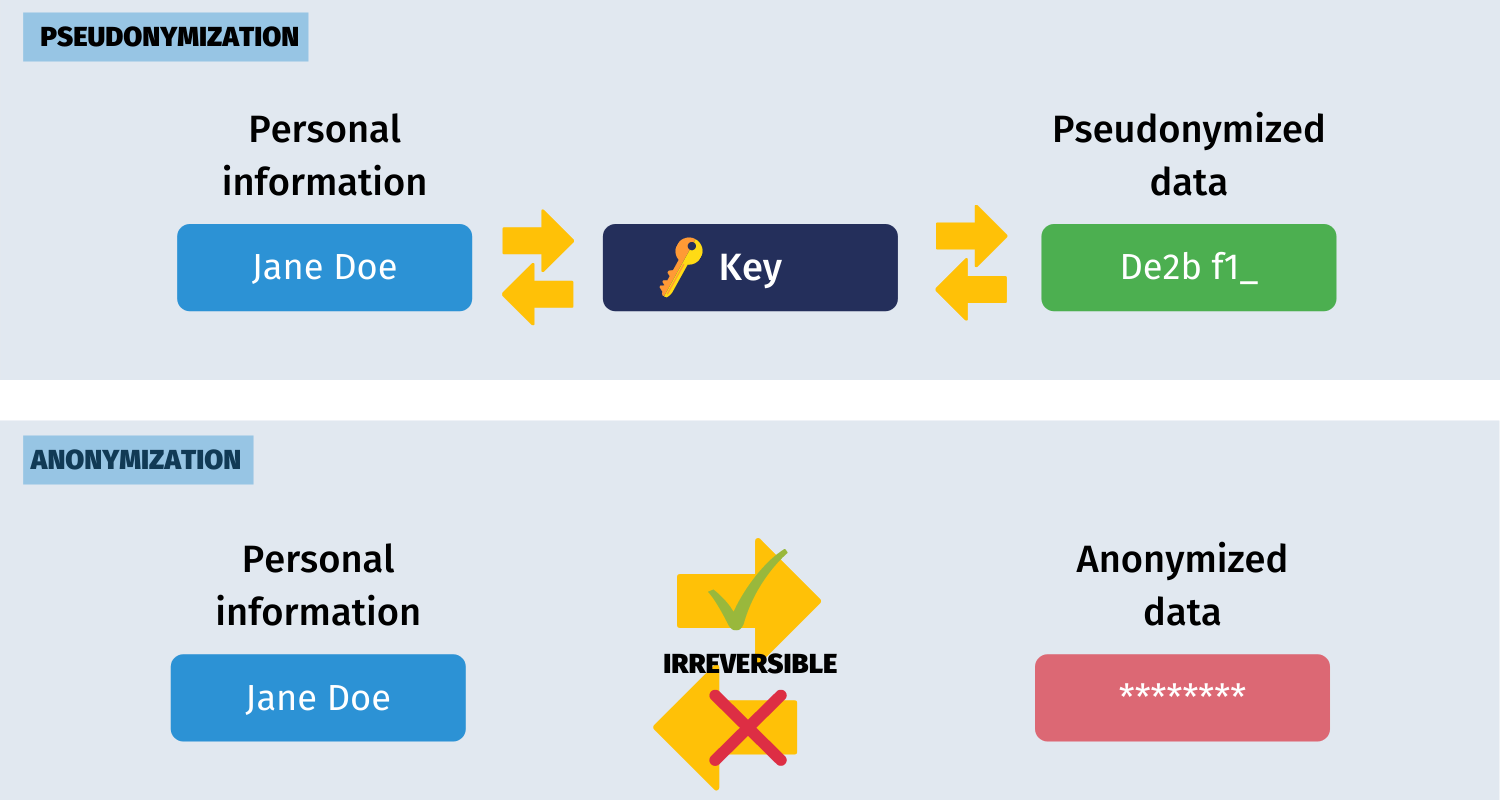
\includegraphics[width=0.8\linewidth]{Images/Difference-between-anonymization-and-pseudonymization.png}
    \caption{Pseudonimizzazione VS Anonimizzazione}
    \label{fig:enter-label}
\end{figure}
 
\chapter{Modello di attacco}

Come detto in precedenza, l'obiettivo principale della pseudonimizzazione è limitare la collegabilità tra un dataset pseudonimizzato e i detentori dei pseudonimi al fine di proteggere l'identità dei soggetti dati. Questo tipo di protezione è generalmente pensato per contrastare i tentativi di un avversario di eseguire un \textbf{attacco di re-identificazione}.

\section{Avversari Interni ed Avversari Esterni}

Questo capitolo considera i possibili modelli di attacco e \textbf{diversi tipi di attacchi di re-identificazione} che sono importanti per la pseudonimizzazione. A tale scopo, vengono esaminati i concetti di avversari interni ed esterni, analizzando i loro possibili ruoli nei scenari di pseudonimizzazione discussi in precedenza nel rapporto. 

\subsection{Avversari Interni}

Secondo la definizione comune nel campo della sicurezza informatica, un \textbf{avversario interno} è una \textbf{persona con conoscenze specifiche}, capacità o permessi (riguardo all'obiettivo dell'avversario). 

Nel contesto della pseudonimizzazione, ciò implica che l'avversario sia in grado di \textbf{ottenere informazioni sul segreto di pseudonimizzazione} e/o altre informazioni significative rilevanti.

Ad esempio, un avversario interno potrebbe essere un dipendente che lavora per il responsabile del trattamento, oppure potrebbe essere situato all'interno di una terza parte fidata (agendo in questo caso come entità di pseudonimizzazione). Per default, le terze parti che potrebbero legittimamente avere accesso ai dati personali (come un'autorità di vigilanza o di forze dell'ordine) non vengono considerate avversarie.

\subsection{Avversari Esterni}

A differenza dell'avversario interno, un avversario esterno\textbf{ non ha accesso diretto al segreto di pseudonimizzazione} o ad altre informazioni rilevanti. Tuttavia, questo tipo di avversario potrebbe \textbf{avere accesso a un dataset pseudonimizzato} e potrebbe essere in grado di \textbf{eseguire il processo di pseudonimizzazione} su valori di input arbitrari scelti dall'avversario.

L'obiettivo di un avversario esterno è aumentare le proprie conoscenze sul dataset pseudonimizzato, come ad esempio scoprire l'identità dietro un determinato pseudonimo e acquisire ulteriori informazioni su tale identità dai dati aggiuntivi presenti nel dataset associati al pseudonimo fornito.


\section{Obiettivi degli Attacchi alla Pseudonimizzazione}

A seconda del contesto e del metodo di pseudonimizzazione utilizzato, l'avversario può avere diversi obiettivi che intende raggiungere nei confronti dei dati pseudonimizzati, come il \textbf{recupero del segreto di pseudonimizzazione}, la \textbf{re-identificazione completa} o la \textbf{discriminazione.} 

\subsection{Segreto di Pseudonimizzazione}

L'avversario si concentra sullo scoprire il segreto di pseudonimizzazione (cioè quando viene utilizzato il segreto di pseudonimizzazione). Questo tipo di attacco è il più grave, poiché \textbf{con il segreto di pseudonimizzazione} l'avversario è in grado di\textbf{ re-identificare qualsiasi pseudonimo} nel dataset (re-identificazione completa o discriminazione), nonché di eseguire ulteriori processi di pseudonimizzazione sul dataset.

\subsection{Re-identificazione Completa}

Quando l'obiettivo dell'attacco è la re-identificazione completa, l'avversario desidera\textbf{ collegare uno o più pseudonimi all'identità dei detentori degli pseudonimi.}

Il più grave attacco di re-identificazione completa consiste nella re-identificazione di tutti gli pseudonimi. 
\\\\
L'avversario può utilizzare due strategie per raggiungere questo obiettivo: 
\begin{itemize}
    \item Recuperare ogni identificatore dal corrispondente pseudonimo indipendentemente 
    \item Recuperare il segreto di pseudonimizzazione
\end{itemize}

La forma meno grave degli attacchi di re-identificazione completa coinvolge un avversario che può solo re-identificare un sottoinsieme di pseudonimi nel dataset.

Ad esempio, consideriamo un dataset pseudonimizzato dei voti degli studenti di un corso universitario. Ogni voce del dataset contiene un pseudonimo corrispondente all'identità dello studente (nome e cognome) e un secondo pseudonimo sul genere dello studente (ad esempio, mappando gli studenti maschi a numeri dispari e le studentesse a numeri pari). Un avversario ha successo in un attacco di re-identificazione completa se riesce a recuperare il nome, il cognome e il genere di uno studente.

\subsection{Discriminazione}

L'obiettivo dell'attacco di discriminazione è \textbf{identificare le proprietà di un detentore di pseudonimo} (almeno una). Queste proprietà potrebbero non portare direttamente alla scoperta dell'identità del detentore dello pseudonimo, ma possono essere sufficienti per discriminare in qualche modo.
È importante capire che l'avversario \textbf{non apprende l'identità del detentore dello pseudonimo} in questo caso, ma\textbf{ solo alcune proprietà}.L'avversario \textbf{non è in grado di individuare l'esatto record} di dati di un determinato detentore di pseudonimo. Tuttavia, le informazioni aggiuntive acquisite possono già essere sufficienti per scopi di discriminazione che l'avversario intende eseguire, o possono essere utilizzate in un successivo attacco di conoscenza di fondo per scoprire l'identità dietro uno pseudonimo.

 
\chapter{Tecniche di pseudonimizzazione}

In linea di principio, una funzione di pseudonimizzazione mappa identificatori in pseudonimi. C'è un requisito fondamentale per una funzione di pseudonimizzazione. Consideriamo due identificatori differenti \( \text{Id}_1 \) e \( \text{Id}_2 \) e i loro pseudonimi corrispondenti \( \text{pseudo}_1 \) e \( \text{pseudo}_2 \). Una funzione di pseudonimizzazione deve verificare che \( \text{pseudo}_1 \) sia diverso da \( \text{pseudo}_2 \). Altrimenti, il recupero dell'identificatore potrebbe essere ambiguo: l'entità di pseudonimizzazione non può determinare se \( \text{pseudo}_1 \) corrisponde a \( \text{Id}_1 \) o \( \text{Id}_2 \). Tuttavia, un singolo identificatore \( \text{Id} \) può essere associato a più pseudonimi \( (\text{pseudo}_1, \text{pseudo}_2, \ldots) \) purché sia possibile per l'entità di pseudonimizzazione invertire questa operazione.

\section{Principali tecniche di Pseudonimizzazione}

\subsection{Contatore}

Il contatore è la\textbf{ funzione di pseudonimizzazione più semplice}, dove gli identificatori vengono sostituiti da un numero incrementato in modo monotono. È adatto per dataset piccoli e non complessi, ma può presentare problemi di implementazione e scalabilità per dataset più grandi.

\subsection{Generatore di numeri casuali (RNG)}

Il generatore di numeri casuali assegna un \textbf{numero casuale agli identificatori}, garantendo che \textbf{ogni pseudonimo sia imprevedibile}. Tuttavia, possono verificarsi collisioni, influenzate dal noto paradosso del compleanno.

\subsection{Funzione hash crittografica}

Una funzione hash crittografica\textbf{ mappa stringhe di lunghezza variabile} in output di \textbf{lunghezza fissa}. Tuttavia, è considerata\textbf{ debole }per la pseudonimizzazione a causa della vulnerabilità a \textbf{attacchi di forza bruta} e \textbf{dizionario.}

\subsection{Codice di autenticazione del messaggio (MAC)}

Il \textbf{MAC} è una \textbf{funzione di hash} con chiave che genera pseudonimi \textbf{utilizzando una chiave segreta}. È robusto dal punto di vista della protezione dei dati, a condizione che la chiave non venga compromessa.

\section{Meccanismi di recupero}

In conformità alla definizione, l'uso di informazioni aggiuntive è fondamentale per la pseudonimizzazione, pertanto l'entità di pseudonimizzazione deve implementare un \textbf{meccanismo di recupero.}
Questa operazione può essere necessaria, ad esempio, quando l'entità di pseudonimizzazione rileva un'anomalia nel sistema e deve contattare le entità designate. Tale "anomalia" potrebbe essere una \textbf{violazione dei dati}, obbligando l'entità di pseudonimizzazione a \textbf{notificare i soggetti dei dati} in base al GDPR. Inoltre, il meccanismo di recupero potrebbe essere necessario per consentire l'esercizio dei diritti dei soggetti dei dati (ai sensi degli articoli 12-21 del GDPR).

\begin{table}[ht]
\centering
\begin{tabular}{|l|l|}
\hline
\textbf{Metodo}              & \textbf{Recupero basato su pseudonimo} \\ \hline
Counter                      & Tabella di mappatura                  \\ \hline
Generatore di numeri casuali & Tabella di mappatura                  \\ \hline
Funzione di hash crittografica  & Tabella di mappatura                  \\ \hline
Codici di autenticazione del messaggio & Tabella di mappatura                  \\ \hline
Crittaggio                   & Decrittazione                         \\ \hline
\end{tabular}
\caption{Confronto tra meccanismi di recupero}
\end{table}



\chapter{Principali tecniche di attacco}

Ci sono\textbf{ tre principali tecniche} generiche per rompere una funzione di pseudonimizzazione: \textbf{attacchi brute force}, ricerca tramite \textbf{dizionario} e\textbf{ tentativi} (guesswork). L'efficacia di questi attacchi dipende da diversi parametri, tra cui:
\begin{itemize}
  \item La\textbf{ quantità di informazioni} sul titolare del pseudonimo (soggetto dei dati) contenuta nel pseudonimo.
  \item La \textbf{conoscenza pregressa dell'avversario}.
  \item La\textbf{ dimensione del dominio} dell'\textbf{identificatore}.
  \item La \textbf{dimensione del dominio} del \textbf{pseudonimo}.
  \item La scelta e l\textbf{a configurazione della funzione di pseudonimizzazione} utilizzata (che include anche la 
  dimensione del segreto di pseudonimizzazione).
\end{itemize}

\section{Attacco brute force}

La praticità di questa tecnica di attacco dipende dalla capacità dell'avversario di \textbf{calcolare la funzione di pseudonimizzazione}. 
A seconda dell'obiettivo dell'attacco, possono applicarsi condizioni aggiuntive. Se l'attacco brute force è utilizzato per ottenere il ripristino dell'identità originale, il dominio dell'identificatore deve essere finito e relativamente piccolo. Per ogni pseudonimo incontrato dall'avversario, questi può tentare di recuperare l'identificatore originale applicando la funzione di pseudonimizzazione su ogni valore del dominio dell'identificatore fino a trovare una corrispondenza.

Consideriamo la\textbf{ pseudonimizzazione del mese di nascita in un dataset}. La dimensione del dominio dell'identificatore è \textbf{12}, quindi un avversario può enumerare rapidamente tutte le possibilità. I pseudonimi associati a ciascun mese sono calcolati in questo caso come la somma del codice ASCII delle prime tre lettere del mese di nascita (con la prima lettera maiuscola). Supponiamo che un avversario incontri il pseudonimo 301. Questo può applicare la funzione di pseudonimizzazione su ogni mese di nascita fino a trovare quello che corrisponde al valore 301. La Tabella 1 mostra i calcoli effettuati dall'avversario per riconoscere il pseudonimo 301, risultando nella tabella di mappatura della funzione di pseudonimizzazione.

\begin{table}[h]
\centering
\begin{tabular}{|c|c|}
\hline
Mese di nascita & Pseudonimo \\
\hline
Gen. & 281 \\
Feb. & 269 \\
Mar. & 288 \\
Apr. & 291 \\
Mag. & 295 \\
Giu. & 301 \\
Lug. & 299 \\
Ago. & 285 \\
Sett. & 296 \\
Ott. & 294 \\
Nov. & 307 \\
Dic. & 268 \\
\hline
\end{tabular}
\caption{Pseudonimizzazione del mese di nascita}
\end{table}

\section{Attacco Dizionario}
La ricerca tramite dizionario è un'\textbf{ottimizzazione dell'attacco brute force}, che può risparmiare costi computazionali. 
Ogni voce nel dizionario contiene un \textbf{pseudonimo} e l'identificatore o l'informazione corrispondente. Ogni volta che l'avversario ha bisogno di riconoscere nuovamente un pseudonimo, cerca nel dizionario. 
La ricerca tramite dizionario consiste essenzialmente nel \textbf{calcolo} e nel \textbf{salvataggio della tabella di mappatura}. Sono possibili compromessi tra tempo e memoria utilizzando tavole di Hellman o tabelle arcobaleno per estendere ulteriormente il range. 

\section{Guesswork}

Questo tipo di attacco\textbf{ utilizza conoscenze pregresse} (come distribuzioni di probabilità o altre informazioni secondarie) che l'avversario può avere su alcuni (o tutti) i titolari di pseudonimi.
Sfruttare le\textbf{ caratteristiche statistiche} degli identificatori è noto come guesswork ed è ampiamente utilizzato nella comunità di cracking delle password. 
L'avversario \textbf{non ha} necessariamente \textbf{bisogno di accedere alla funzione di pseudonimizzazione} (poiché la discriminazione è possibile semplicemente eseguendo un'analisi della frequenza dei pseudonimi osservati).

Consideriamo un caso che riguarda i pseudonimi corrispondenti ai "nomi propri". Esplorare completamente il dominio dei "nomi propri" è difficile. Tuttavia, l'avversario sa quali "nomi propri" sono i più popolari. L'avversario può eseguire una ricerca esaustiva o una ricerca tramite dizionario nel dominio dei "nomi propri" più popolari e ottenere la discriminazione.

\begin{table}[h]
\centering
\begin{tabular}{|c|}
\hline
Nomi propri più popolari \\
\hline
Bob \\
Alice \\
Charlie \\
Eve \\
Robert \\
Marie \\
\hline
\end{tabular}
\caption{Lista di nomi propri più popolari}
\end{table}

A seconda della quantità di informazioni di background o metadati di cui dispone l'avversario e della quantità di informazioni collegabili trovate nel dataset pseudonimizzato, questo tipo di attacco può portare a scoprire l'identità di un singolo titolare di pseudonimo, una frazione di essi o l'intero dataset. Specialmente per dataset piccoli, tali attacchi possono essere fattibili con alti tassi di successo.


\chapter{Principali meccanismi di difesa}

\section{Cos'è un attacco di re-identificazione?}

Gli attacchi di re-identificazione sono metodi per de-anonimizzare i dati utilizzando informazioni aggiuntive, come database esterni, metadati o analisi statistica, per inferire le identità dei soggetti dei dati. Gli attacchi di re-identificazione possono essere classificati in tre tipi principali:

\begin{itemize}
    \item \textbf{Attacchi di collegamento (linking attack):} Coinvolgono il match di dati anonimizzati con altre fonti di dati che contengono informazioni identificative, come nomi, indirizzi o numeri di telefono.
    \item \textbf{Attacchi di inferenza (inference attack):} Basati sull'uso di metodi statistici o di apprendimento automatico per dedurre informazioni sensibili dai dati anonimizzati, come genere, età o stato di salute.
    \item \textbf{Attacchi di ricostruzione:} I più avanzati, utilizzano dati anonimizzati da più fonti o interrogazioni per ricostruire i dati originali o una loro approssimazione.
\end{itemize}

\section{Come prevenire gli attacchi di collegamento?}

Utilizzare \textbf{tecniche robuste di anonimizzazione} per garantire che ogni record anonimizzato sia indistinguibile dagli altri e che ogni gruppo di record abbia una diversità sufficiente di valori sensibili.

\section{Come prevenire gli attacchi di inferenza?}

Utilizzare l'\textbf{iniezione di rumore} per aggiungere\textbf{ errori casuali o controllati ai dati}, riducendo così la loro precisione e utilità per gli attaccanti. Applicare la privacy differenziale per garantire che la presenza o l'assenza di un individuo nei dati non influenzi l'esito delle analisi. Limitare la \textbf{quantità} e la\textbf{ granularità dei dati condivisi} e utilizzare meccanismi di controllo degli accessi e crittografia.

\section{Come prevenire gli attacchi di ricostruzione?}

Utilizzare la computazione sicura multiparte per consentire a più parti di eseguire calcoli sui loro dati senza rivelarli tra loro o a terzi. Adottare la crittografia omomorfica per eseguire operazioni su dati crittografati senza decifrarli. Sfruttare il learning federato per apprendere da dati locali in modo distribuito senza centralizzarli.



\chapter{Sperimentazione di attacco}

\chapter*{Conclusione} %l'asterisco dopo chapter serve per visualizzare il capitolo come "non numerato"
\addcontentsline{toc}{chapter}{Conclusione} %per fare inserire il capitolo nella tabella dei contenuti
 %<- richiama il file "parts/conclusione.tex" che contiene la conclusione

\chapter*{Glossario}

\section*{Dati Personali}
Si riferisce a qualsiasi informazione relativa a una persona fisica identificata o identificabile (interessato); una persona fisica identificabile è colui che può essere identificato, direttamente o indirettamente, in particolare mediante un identificativo come nome, numero di identificazione, dati di localizzazione, identificativo online o uno o più fattori specifici della identità fisica, fisiologica, genetica, mentale, economica, culturale o sociale di quella persona (GDPR, art. 4(1)).

\section*{Responsabile del Trattamento}
Persona fisica o giuridica, autorità pubblica, agenzia o altro ente che, da solo o congiuntamente ad altri, determina le finalità e i mezzi del trattamento dei dati personali (GDPR, art. 4(7)).

\section*{Responsabile del Trattamento}
Persona fisica o giuridica, autorità pubblica, agenzia o altro ente che tratta dati personali per conto del titolare del trattamento (GDPR, art. 4(8)).

\section*{Pseudonimizzazione}
Il trattamento dei dati personali in modo tale che i dati personali non possano più essere attribuiti a un soggetto specifico senza l'uso di informazioni aggiuntive, a condizione che tali informazioni aggiuntive siano conservate separatamente e siano soggette a misure tecniche e organizzative per garantire che i dati personali non siano attribuibili a una persona fisica identificata o identificabile (GDPR, art. 4(5)).

\section*{Anonimizzazione}
Un processo mediante il quale i dati personali vengono alterati in modo irreversibile in modo che un soggetto non possa essere più identificato direttamente o indirettamente, né dal titolare del trattamento da solo né in collaborazione con altre parti (ISO/TS 25237:2017).

\section*{Identificativo}
Un valore che identifica un elemento all'interno di uno schema di identificazione. Un identificativo univoco è associato a un solo elemento.

\section*{Pseudonimo}
Conosciuto anche come criptonimo o semplicemente nym, è un pezzo di informazione associato a un identificativo di un individuo o a qualsiasi altro tipo di dato personale (ad esempio, dati di localizzazione). I pseudonimi possono avere diversi gradi di collegabilità agli identificativi originali.

\section*{Avversario}
Un ente che cerca di rompere la pseudonimizzazione e collegare un pseudonimo (o un dataset pseudonimizzato) al detentore del pseudonimo.

\section*{Attacco di Re-identificazione}
Un attacco alla pseudonimizzazione eseguito da un avversario che mira a ri-identificare il detentore di un pseudonimo.
 %<- richiama il file "parts/conclusione.tex" che contiene la conclusione

%Inserisce la bibliografia
\addcontentsline{toc}{chapter}{Bibliografia} %per fare inserire il capitolo nella tabella dei contenuti

\begin{thebibliography}{9}

\bibitem{pseudonymizationGDPR}
  Data Privacy Manager,
  \textit{Pseudonymization according to the GDPR},
  [Online]. Available: \url{https://dataprivacymanager.net/pseudonymization-according-to-the-gdpr/}. 

\bibitem{ENISA2021}
  ENISA,
  \textit{Pseudonymisation Techniques and Best Practices},
  [Online]. Available: \url{https://www.enisa.europa.eu/publications/pseudonymisation-techniques-and-best-practices}.

\bibitem{Pseudonymization Defense}
  LinkedIn,
  \textit{How Can You Protect Against Re-identification Attacks},
  [Online]. Available: \url{  https://www.linkedin.com/advice/0/how-can-you-protect-against-re-identification-attacks}.

\bibitem{Data re-identification}
  Wikipedia,
  \textit{Data Re-Identification},
  [Online]. Available: \url{https://en.wikipedia.org/wiki/Data_re-identification}.

\bibitem{Guidelines of Pseudonymization}
  NewSchool,
  \textit{Guidelines Anonymization and Pseudonymization},
  [Online]. Available: \url{https://ispo.newschool.edu/guidelines/anonymization-pseudonymization/}.

\bibitem{Privacy by Evidence}
  Research Gate,
  \textit{Develop Privacy Friendly Software},
  [Online]. Available: \url{https://www.researchgate.net/publication/336043425_Privacy_by_Evidence_A_Methodology_to_Develop_Privacy-Friendly_Software_Applicationsn}.

\bibitem{Kaggle Healthcare Dataset}
  Kaggle,
  \textit{Healthcare Dataset},
  [Online]. Available: \url{https://www.kaggle.com/datasets/prasad22/healthcare-dataset?resource=download}.
  
\end{thebibliography} %<- richiama il file "parts/conclusione.tex" che contiene la conclusione

\end{document}